% !TeX encoding = utf8
% !TeX program = xelatex
% -*- coding:utf-8 mod:LaTeX -*-

% Paper 5: Task-Oriented SC-BSS
% Template: elsarticle (review format) — target venue: AEÜ — Int. J. of
% Electronics and Communications (Elsevier)

\documentclass[review,12pt]{elsarticle}

\usepackage{graphicx}
\usepackage{booktabs}
\usepackage{amsmath,amssymb}
\usepackage{url}
\usepackage{xcolor}
\usepackage[mode=text]{siunitx}
\sisetup{locale=US}

\usepackage{hyperref}
\hypersetup{hidelinks,
  colorlinks=true,
  allcolors=black,
  pdfstartview=Fit,
  breaklinks=true}

\usepackage{lineno}
\modulolinenumbers[5]

\usepackage{float}

\emergencystretch=1.5em

\newcommand{\snr}{\mathrm{SNR}}
\newcommand{\sir}{\mathrm{SIR}}

\journal{AE\"U -- International Journal of Electronics and Communications}

\begin{document}

\begin{frontmatter}

\title{Task-Oriented Single-Channel Blind Source Separation:\\Bit-Level
Gains Are Interference-Limited, Not Loss-Limited}

\author[1]{Bin Nong\corref{cor1}}
\ead{nongbin@tfswufe.edu.cn}
\author[2]{Weihong Fu}
\author[3]{Zhuoyun Jiang}

\affiliation[1]{organization={Tianfu College of Southwestern University of Finance and Economics}, city={Mianyang}, state={Sichuan}, postcode={621000}, country={China}}
\affiliation[2]{organization={School of Telecommunications Engineering, Xidian University}, city={Xi'an}, state={Shaanxi}, postcode={710071}, country={China}}
\affiliation[3]{organization={School of Health Science and Engineering, University of Shanghai for Science and Technology}, city={Shanghai}, postcode={200093}, country={China}}

\cortext[cor1]{Corresponding author.}

% ======================================================================
\begin{abstract}
Single-channel blind source separation (SC-BSS) of co-frequency
communication signals is trained and ranked almost exclusively by
waveform-fidelity metrics such as the scale-invariant
signal-to-distortion ratio (SI-SDR), yet the downstream task is
demodulation. On a variable-count ($K \in \{1,2,3\}$)
benchmark evaluated with an offset-compensated receiver (oracle carrier
synchronisation, matched filtering, Gray-mapped bit error rate, BER), we quantify
the mismatch: a $+4.1$\,dB SI-SDR improvement moves the compensated
symbol error rate (SER) from 0.5049 to 0.5027---even $+8.4$\,dB at
$-10$\,dB SNR buys nothing---if anything it costs a fraction of a
point---because the mixture is interference-limited at
$\mathrm{SIR} \approx 0$\,dB. We then test a \emph{task-oriented
loss}: a differentiable soft-demodulation term line-by-line
identical to the evaluation receiver,
inserted into the variable-$K$ permutation-invariant loss. The pooled
bit-level effect across five seeds is practically negligible (at most
0.03 percentage points (pp) in the fair additive comparison) but hides a sign
structure along the interference axis: the term \emph{helps} at $K{=}2$
(BER $+0.06$ to $+0.40$\,pp across contrasts, 5/5 seeds positive in all
four) and \emph{hurts} at $K{=}3$ (SER $-0.6$ to $-0.7$\,pp,
0/5 seeds positive in all four), so the number of interferers, not the
loss, sets its sign. Removing the waveform
objective entirely collapses the model (reward hacking of the soft
receiver; SI-SDRi $-9.4$\,dB): waveform supervision is necessary but
not sufficient. The task term also regularises source counting
(occupancy-routed count accuracy $0.65 \rightarrow 0.85$; hallucination
$0.15 \rightarrow 0.05$--$0.06$). A joint soft-information head bypassing
explicit separation fails at chance level; a controlled
probe attributes the failure to burst-level blind carrier/phase
recovery. Closing the waveform-to-bit gap requires explicit
synchronisation and equalisation structure, not a better loss weight.
\end{abstract}

\begin{keyword}
Blind source separation \sep Co-frequency communication \sep
Task-oriented learning \sep Symbol error rate \sep Soft demodulation
\sep Complex-valued neural network
\end{keyword}

\end{frontmatter}

\linenumbers

% ======================================================================
\section{Introduction}
\label{sec:intro}

\emph{Problem and motivation.} Single-channel blind source separation
(SC-BSS) recovers multiple unknown source signals from one observed
mixture~\cite{hou2022single,guo2024single}. For co-frequency
communication signals---several modulated emitters overlapping in time
and frequency at a single receiving antenna---deep separators have
progressed along a clear axis: better architectures, trained and ranked
by waveform-fidelity metrics, above all the scale-invariant
signal-to-distortion ratio (SI-SDR)~\cite{kolbaek2017pit,leroux2019sdr}
and its improvement over the mixture (SI-SDRi). Yet separation is rarely
the end goal. In spectrum monitoring, cognitive radio and electronic
support, the separated waveforms are fed to a \emph{demodulator}, and
the quantity the operator pays for is the bit error rate (BER). The
premise of the whole line of work is that waveform fidelity is a good
proxy for bit-level recoverability. This paper tests that premise
directly, finds it wanting, and then tests the obvious remedy---training
the separator on a differentiable demodulation loss---with equal care.

\emph{Why the premise is fragile here.} Two properties of the
co-frequency setting conspire against the proxy. First, SI-SDR is
scale- and phase-invariant: it does not care whether the estimated
waveform lands on the constellation grid that a demodulator's decision
boundaries carve out. Second, the practically relevant operating point
of a co-frequency mixture is symmetric interference: with comparable
per-source amplitudes the signal-to-interference ratio is
$\sir \approx 0$\,dB, so the residual on any separated output is not
small receiver noise but \emph{amplitude-level leakage of the other
sources}. Whether any training objective can push a separated waveform
across decision boundaries under such residuals is an empirical question
that, to our knowledge, has not been answered with statistically
controlled experiments.

\emph{What we do.} We work on a variable-count co-frequency SC-BSS
benchmark ($K \in \{1,2,3\}$ sources; BPSK/QPSK/8PSK/16QAM;
root-raised-cosine pulses; multipath fading; AWGN) inherited from our
companion open-world study~\cite{nong2026openworld}, and evaluate every
model with an \emph{offset-compensated receiver}: oracle down-conversion
at each source's true carrier, matched filtering, unit-power symbol
grid, phase-only alignment, minimum-distance decisions, and Gray-mapped
BER from the same decisions (Section~\ref{sec:truth}). On top of this
evaluation truth we build a \emph{differentiable soft-demodulation
loss} whose receiver front-end is line-by-line identical to the
evaluation receiver, and insert it into the variable-$K$
permutation-invariant training (PIT) loss (Section~\ref{sec:method}).
Three studies follow. S1 quantifies the SI-SDR$\,\to\,$SER/BER mismatch
on fifteen previously trained separators. S2 trains the same slot
separator under five loss configurations (five seeds each) with exact
and Monte-Carlo permutation tests. S3 attempts the classical end of the
task-oriented road---a joint soft-information head that bypasses the
explicit waveform stage---and diagnoses its failure with a controlled
synchronisation probe.

\emph{Findings.}
\begin{enumerate}
  \item \textbf{The mismatch is real and large.} $+4.1$\,dB SI-SDRi
        moves the compensated SER from 0.5049 (mixture, no separation)
        to 0.5027 and the Gray BER from 0.2669 to 0.2651; even
        $+8.4$\,dB SI-SDRi at $-10$\,dB SNR buys nothing (a
        fraction-of-a-point penalty, if anything), and the flatness
        persists across an SIR sweep to $20$\,dB at fixed $K{=}2$
        (Section~\ref{sec:s1}). The damage localises to interference:
        the baseline SER jumps from 0.146 at $K{=}1$ to 0.561 at
        $K{=}2$ and only 0.587 at $K{=}3$---one interferer closes
        nearly the whole demodulation gap.
  \item \textbf{A faithfully aligned task loss barely moves it, and
        the sign is set by the interference, not the loss.} Pooled
        over $K$, the soft-SER term is practically negligible
        ($\leq 0.17$\,pp BER for the replacement configuration (c);
        $\leq 0.03$\,pp for the fair additive comparison (d) vs.\ (b)).
        Decomposed by source count, however, the term \emph{helps} at
        $K{=}2$---the $\sir \approx 0$\,dB case that motivates it
        (BER $+0.35$\,pp for the replacement contrast, $+0.11$\,pp in
        the fair additive one, 5/5 seeds in all four contrasts, exact
        permutation $p = 0.0625$)---and \emph{hurts} at $K{=}3$ (SER
        $-0.6$ to $-0.7$\,pp, 0/5 seeds in all four contrasts), the two
        cancelling in the pool (Section~\ref{sec:s2}).
  \item \textbf{Waveform supervision is necessary but not sufficient.}
        A pure soft-SER loss finds off-manifold solutions that minimise
        the soft receiver's cross-entropy without separating
        (SI-SDRi $-9.4$\,dB, SER \emph{worse} than the unseparated
        mixture)---a reward-hacking failure that also delimits where the
        training proxy can be trusted (Section~\ref{sec:abl}).
  \item \textbf{The task term is not useless---it regularises the
        occupancy structure.} Occupancy-routed count accuracy rises from
        0.65 to 0.85 and the hallucination rate drops from 0.15 to
        0.05--0.06,
        an emergent benefit for the slot \emph{gating} that waveform
        losses do not provide (a dedicated count head, at $\approx$0.9
        ($0.87$--$0.92$) for
        all configurations, still counts better---the gain is in what
        the gates pass downstream, not in the count itself;
        Sections~\ref{sec:s2} and~\ref{sec:abl}).
  \item \textbf{Naive joint detection fails, informatively.} A learned
        per-symbol posterior head sits at the chance level, and
        controlled probes (same head, same data, oracle vs.\ blind
        synchronisation) point to burst-level blind carrier/phase
        recovery as the binding constraint at $K{=}1$; at $K{=}2$ even
        a frequency oracle fails to beat the mixture baseline---sync
        alone is not sufficient under phase entanglement
        (Section~\ref{sec:s3}).
\end{enumerate}

The overall picture these results support is mechanistic, not
statistical-anecdotal: the residual on any separated output is
interference leakage, and what a grid-aware task loss can add on top of
a waveform loss depends on the \emph{structure} of that leakage---one
interferer's residue is structured enough to nudge across decision
boundaries ($K{=}2$), two interferers' residue fills the grid and turns
the same gradient misleading ($K{=}3$). Closing the gap requires
explicit synchronisation and equalisation structure in the model, not a
re-weighted loss. Section~\ref{sec:disc} develops this argument.

The remainder of the paper is organised as follows.
Section~\ref{sec:related} reviews the literature this work connects.
Section~\ref{sec:truth} defines the benchmark and the compensated
receiver that serves as evaluation truth. Section~\ref{sec:method}
describes the separator, the differentiable soft-demodulation loss, and
the joint head. Section~\ref{sec:exp} presents S1--S3.
Section~\ref{sec:disc} gives the mechanistic discussion,
Section~\ref{sec:limit} states limitations, and
Section~\ref{sec:concl} concludes.

% ======================================================================
\section{Related Work}
\label{sec:related}

\subsection{SC-BSS for communication signals}

Blind separation of co-frequency communication signals from a single
sensor violates the overdetermined requirement of classical
ICA~\cite{hyvarinen2000ica}; classical workarounds exploit
time--frequency sparsity in the underdetermined
case~\cite{su2017underdetermined}, and the co-frequency setting
has driven a line of deep-learning
approaches: convolutional separation networks~\cite{hou2022single},
recurrent designs~\cite{chen2019deep}, attention-augmented
models~\cite{ma2023novel}, complex-domain
architectures~\cite{guo2024single}, spatial-temporal
fusion~\cite{luo2023single}, and structured state-space
backbones~\cite{s4unet2026}. The setting has recently been extended to
an unknown number of sources by coupling separation with source
counting, in radar mixtures~\cite{edsnet2026} and in our companion
open-world study~\cite{nong2026openworld}, whose variable-$K$ benchmark,
slot architecture and trained checkpoints this paper builds on. All of
these works train and rank models by waveform metrics (SI-SDR, SDR,
NMSE); bit-level read-outs under a compensated receiver are rare, and to
our knowledge no prior work tests whether waveform improvements reach
the demodulated bits under symmetric co-frequency mixtures---the
question addressed here.

\subsection{Waveform metrics and their discontents}

Modern time-domain separation descends from deep
clustering~\cite{hershey2016deep}, PIT~\cite{kolbaek2017pit} and
Conv-TasNet~\cite{luo2019conv}, with SI-SDR as the dominant training
and reporting metric. That the metric is not the task is well documented
in audio: the BSS\_EVAL suite itself warns that energy-ratio metrics
conflate artefacts with interference~\cite{vincent2006bsseval}, and
Le~Roux et al.~\cite{leroux2019sdr} show that SI-SDR improvements can
be purchased with distortions the metric cannot see, recommending
task-level evaluation. We import this scepticism to co-frequency
\emph{communication} mixtures, where the task metric is sharp and
unambiguous---symbol and bit error rate under a compensated
receiver---and quantify the mismatch rather than assuming it.

\subsection{Task-oriented and semantic communication}

Task-oriented communication argues that transmit and receive processing
should be optimised for the consumer of the message rather than for
reconstruction
fidelity~\cite{strinati2021semantic,gunduz2023beyond}, and deep learning
for the physical layer has made end-to-end learned transceivers
practical~\cite{oshea2017intro}. In speech enhancement the principle
delivers: metric-oriented adversarial training and joint acoustic-model
training of separation front-ends improve downstream recognition where
waveform metrics plateau~\cite{lo2019metricgan,ochiai2017multichannel}.
Our work is complementary and, in a sense, cautionary: we apply the
task-oriented principle to the \emph{separation} stage of a receiver
chain for co-frequency communication mixtures, and find that there the
principle is bounded by the interference structure of the channel---the
attainable bit-level gain is set by the number of interferers, not by
the loss.

\subsection{Learned detection and joint demodulation}

That joint multiuser detection outperforms separate-then-detect
pipelines is classical~\cite{verdu1998multiuser}, and practical
co-channel systems have long exploited exactly that structure:
paired-carrier multiple access (PCMA) lets two transmitters share one
carrier and separates them at the receiver with explicit
synchronisation, channel estimation and self-interference
cancellation~\cite{dankberg1998pcma}, while two decades of
interference-cancellation receiver design treat explicit synchronisation
and equalisation as the irreducible core of co-channel
demodulation~\cite{andrews2005interference}. Neural approximations
of multiuser detectors learn the detection mapping
directly~\cite{samuel2019learning,farsad2018neural}, but assume
symbol-synchronous, equalised inputs and (typically) known channel
state---the synchronisation problem is solved before the network sees
the signal. Our S3 experiment asks whether a lightweight head attached
to a separation backbone can absorb joint detection \emph{and}
burst-level synchronisation at once; the answer, with a controlled
probe, is that it cannot (Section~\ref{sec:s3})---consistent with what
those classical designs presuppose.

% ======================================================================
\section{Benchmark and Evaluation Truth}
\label{sec:truth}

\subsection{Variable-$K$ co-frequency mixtures}
\label{sec:setup}

We observe a single complex baseband mixture of $K$ co-frequency
sources,
\begin{equation}
  y(t) = \sum_{k=1}^{K} w_k\, s_k(t) + n(t), \qquad t = 0,\dots,T{-}1,
  \label{eq:mix}
\end{equation}
with $K \in \{1,2,3\}$ drawn uniformly during training (a $K{=}4$
zero-shot probe cell exists in the test grid but is excluded from all
bit-level analyses). Each source $s_k$ is a burst of $N = 256$ symbols
from a modulation alphabet
$m_k \in \{$BPSK, QPSK, 8PSK, 16QAM$\}$, pulse-shaped by a
root-raised-cosine (RRC) filter (roll-off 0.35, 65 taps, a four-symbol
span) at 16 samples
per symbol, passed through a three-tap multipath fading channel, and
carried at $f_k = \SI{2000}{Hz} + \delta_k$ with
$\delta_k \sim \mathcal{U}(0, 5)$\,Hz plus an independent
$\pm \SI{5}{Hz}$ jitter: the sources overlap in both time and
(near-)frequency. The mixture length is $T = 4096$ samples at
$f_s = \SI{16}{kHz}$. Mixing weights are drawn as
$w_k \sim \mathcal{U}(0.4, 0.6)$ (unnormalised), so every multi-source
cell sits at $\sir \approx 0$\,dB by construction---the symmetric,
maximally hostile case. The SNR is defined on total mixture power;
training SNR is uniform in $[-5, 20]$ dB and the test grid spans
$\{-10, -5, \dots, 20\}$ dB. Test sets are deterministic (seed 99999)
with 100 mixtures per (SNR, $K$) cell. The generator is released with
the code; no external dataset is required.

\subsection{The offset-compensated receiver}
\label{sec:rx}

Because the sources sit at \emph{unknown} carrier offsets and the raw
waveform metrics are scale-invariant, a naive demodulation proxy
(nominal-carrier down-conversion, no timing or scale correction) is
defective: fed the \emph{true} 16QAM source waveform it scores SER
$0.92$ ($0.77$ with unit-power normalisation), against $0.000$ for the
compensated receiver (\texttt{check\_naive\_proxy.py}; 253 deterministic
test sources, seed 99999). All bit-level numbers in this paper therefore come
from an \emph{offset-compensated} receiver, applied identically to the
estimate $\hat{s}$ and the reference $s$ of each matched pair:
\begin{enumerate}
  \item \textbf{Oracle down-conversion} at the pair's true carrier
        $f_k$ (exposed by the generator): $\tilde{x}(t) = x(t)\,
        e^{-j 2 \pi f_k t / f_s}$;
  \item \textbf{Matched filtering} with the same RRC taps
        (zero-delay `same' convolution);
  \item \textbf{Symbol-grid sampling} at offset 0 with stride 16 (the
        pipeline's net symbol delay is zero);
  \item \textbf{Unit-power normalisation} of each symbol stream,
        placing both signals on a common grid;
  \item \textbf{Phase-only alignment} of the estimate to the reference:
        $\hat{z} \leftarrow \hat{z}\, e^{j \angle \rho}$ with
        $\rho = \langle z_{\mathrm{ref}}, \hat{z} \rangle /
        \|\hat{z}\|^2$ fitted over all 256 symbols of the burst;
  \item \textbf{Minimum-distance decisions} on the shared grid.
\end{enumerate}
The compensated SER is the symbol-agreement rate of the two decision
sequences; identity input scores $0.000$ on all four modulations, and
clean-source decisions reproduce the transmitted symbols up to a small
multipath-ISI residual that sets the per-modulation \emph{clean floors}
(0.000/0.000/0.014/0.032 for BPSK/QPSK/8PSK/16QAM). Timing is fixed at
the nominal grid (no per-pair timing search), so the metric still
measures waveform fidelity under ideal synchronisation rather than a
production receiver---an \emph{upper-bound} demodulation truth. This
oracle assumption applies to the training loss of
Section~\ref{sec:loss} as well; we return to its implications in
Sections~\ref{sec:s3} and~\ref{sec:limit}.

\subsection{Gray-mapped BER}
\label{sec:ber}

The generator draws symbols directly as constellation points (no bit
stream), so BER is \emph{defined} post-hoc: each decided symbol index
maps to a Gray bit string (BPSK sign bit; QPSK I/Q sign bits;
binary-reflected Gray on the 8PSK ring; per-axis Gray on 16QAM), and
BER is the fraction of mismatched bit positions between the estimate's
and the reference's decision bits. Formally, with
$c_n^{*}, \hat{c}_n \in \mathcal{C}_m$ the reference and estimated
decisions of symbol $n$ and $g(\cdot)$ the Gray map,
\begin{equation}
  \mathrm{SER} = \frac{1}{N} \sum_{n=1}^{N}
  \mathbb{1}\!\left[\hat{c}_n \neq c_n^{*}\right],
  \qquad
  \mathrm{BER} = \frac{1}{N \log_2 M} \sum_{n=1}^{N}
  d_{\mathrm{H}}\!\left(g(\hat{c}_n),\, g(c_n^{*})\right),
  \label{eq:serber}
\end{equation}
where $d_{\mathrm{H}}$ is the Hamming distance.
Every nearest-neighbour pair of
constellation points differs in exactly one bit (verified in the code's
smoke test). SER and BER always come from the \emph{same} decisions.

% ======================================================================
\section{Method: Task-Oriented Training}
\label{sec:method}

\subsection{Slot separator}
\label{sec:arch}

The separator is the slot-occupancy model of~\cite{nong2026openworld}:
a lightweight complex-valued CNN (complex convolutions implemented as
paired real operations~\cite{trabelsi2018complex}) with complex
squeeze-and-excitation channel attention~\cite{hu2018senet} encodes the
mixture into a $64$-channel bottleneck; a decoder produces $K_{\max}=4$
complex masks, each modulating the mixture into one \emph{slot} output;
a shared occupancy head scores each slot as active/empty, and a count
head predicts $K$ directly. At inference, slots whose occupancy
probability exceeds 0.5 are declared active; the occupancy route (count
$=$ number of active slots) is the counting convention used throughout
this paper. The model has $\sim$254K parameters. The architecture is
inherited unchanged; the contributions of this paper are the loss, the
evaluation protocol, and the analysis.

\subsection{A differentiable soft-demodulation loss}
\label{sec:loss}

The task-oriented term must satisfy one requirement above all: the
training proxy and the evaluation truth must be the \emph{same
receiver}, or a null result proves nothing. We therefore implement the
compensated receiver of Section~\ref{sec:rx} as a differentiable torch
pipeline and replace only its final hard decision by a soft
cross-entropy. Concretely, for each PIT-assigned estimate/reference pair
$(\hat{s}, s)$ with true carrier $f_k$ and modulation index $m$, the
front-end of Section~\ref{sec:rx} steps 1--4 produces unit-power symbol
streams $\hat{z}, z \in \mathbb{C}^{N}$; the alignment coefficient
$\rho$ is fitted on \emph{detached} tensors and applied as a fixed
rotation $\hat{z} \leftarrow \hat{z}\, \rho / |\rho|$ (gradients flow
through $\hat{z}$ but not through the fit, so the alignment itself
cannot become a gradient exploit). Soft log-likelihoods over the
per-sample constellation $\mathcal{C}_m$ are
\begin{equation}
  \ell_n(c) = -\frac{|\hat{z}_n - c|^2}{\sigma^2},
  \qquad c \in \mathcal{C}_m,\; n = 1,\dots,N,
  \label{eq:softlogit}
\end{equation}
with softness $\sigma^2 = 0.1$ on the unit-power grid, and the loss is
the cross-entropy of $\mathrm{softmax}(\ell_n)$ against the reference's
hard decision $c_n^{*} = \arg\min_{c \in \mathcal{C}_m} |z_n - c|$
(detached). Note that the logits are computed from the phase-aligned
estimate while the labels come from the unaligned reference: the
reference is the ground truth and needs no alignment---the same
convention as the evaluation receiver. The total training loss is
\begin{equation}
  \mathcal{L} =
  \lambda_{\mathrm{sep}}\,\mathcal{L}_{\text{-SI-SDR}}^{\mathrm{PIT}}
  + \lambda_{\mathrm{occ}}\,\mathcal{L}_{\mathrm{BCE}}
  + \lambda_{\mathrm{cnt}}\,\mathcal{L}_{\mathrm{CE}}
  + \lambda_{\mathrm{mse}}\,\mathcal{L}_{\mathrm{MSE}}
  + \lambda_{\mathrm{ser}}\,\mathcal{L}_{\mathrm{soft\text{-}SER}},
  \label{eq:loss}
\end{equation}
where the SI-SDR term is permutation-invariant over the $K$ true
sources: with the scale-invariant signal-to-distortion ratio
\begin{equation}
  \mathrm{SI\text{-}SDR}(\hat{s}, s) =
  10 \log_{10} \frac{\|\alpha s\|^2}{\|\alpha s - \hat{s}\|^2},
  \qquad
  \alpha = \frac{\langle \hat{s}, s \rangle}{\|s\|^2},
  \label{eq:sisdr}
\end{equation}
(computed on zero-meaned $\hat{s}$ and $s$, as in the implementation),
and $\Pi_K$ the injective assignments of $K$ true sources to the
$K_{\max}$ slots,
\begin{equation}
  \mathcal{L}_{\text{-SI-SDR}}^{\mathrm{PIT}} =
  \min_{\pi \in \Pi_K} \frac{1}{K} \sum_{k=1}^{K}
  \big(-\mathrm{SI\text{-}SDR}(\hat{s}_{\pi(k)},\, s_k)\big),
  \label{eq:pit}
\end{equation}
enumerated exactly ($4$/$12$/$24$ assignments for $K = 1/2/3$).
The MSE anchor (which fixes the output scale that pure SI-SDR
leaves free) and the soft-SER term are computed on the \emph{same}
PIT assignment---no second enumeration---and
$\lambda_{\mathrm{occ}} = 1$, $\lambda_{\mathrm{cnt}} = 0.1$ follow the
companion recipe~\cite{nong2026openworld}.

Proxy--truth parity is enforced, not assumed: on clean sources the hard
version of the torch pipeline (argmax of Eq.~\eqref{eq:softlogit})
reproduces the numpy evaluation receiver's decisions
\emph{symbol-for-symbol}, and the matched filter matches
\texttt{np.convolve} to a relative error of $3.5\times10^{-7}$. The
identity cross-entropy is small but nonzero ($\leq 0.45$, 16QAM worst,
from the multipath-ISI residual) while a mismatched reference scores
11--18---the proxy thus carries a deliberate gradient signal toward the
grid even for a perfect waveform estimate, with a $\geq 4\times$
discriminative margin.

\subsection{Training configurations}
\label{sec:configs}

Five configurations isolate the role of each term of
Eq.~\eqref{eq:loss} ($\lambda_{\mathrm{occ}} = 1$ and
$\lambda_{\mathrm{cnt}} = 0.1$ are always on; only the three terms below
vary, and all keep the $\lambda_{\mathrm{sep}}$-SI-SDR PIT term unless
noted):
\begin{itemize}
  \item[\textbf{(a)}] \textbf{SI-SDR}: $\lambda_{\mathrm{sep}} = 1$,
        nothing else---the paper-1-style baseline;
  \item[\textbf{(b)}] \textbf{MSE}: (a) $+\ \lambda_{\mathrm{mse}} = 1$---the
        companion study's converged recipe~\cite{nong2026openworld};
  \item[\textbf{(c)}] \textbf{soft-SER}: (a) $+\ \lambda_{\mathrm{ser}} = 1$,
        $\lambda_{\mathrm{mse}} = 0$---the task-oriented proposal; note
        that (c) \emph{replaces} the MSE anchor, so the fair
        \emph{additive} comparison is (d) vs.\ (b), not (c) vs.\ (b);
  \item[\textbf{(d)}] \textbf{soft-SER + MSE}: (a) $+\ \lambda_{\mathrm{ser}}
        = 1 + \lambda_{\mathrm{mse}} = 1$---combination;
  \item[\textbf{(e)}] \textbf{pure soft-SER}: $\lambda_{\mathrm{sep}} = 0$,
        $\lambda_{\mathrm{ser}} = 1$---no waveform objective at all
        (single-seed probe; checkpoint selection switches to validation
        soft-SER, since val SI-SDR is meaningless without the waveform
        term).
\end{itemize}

\subsection{Joint soft-information head (S3)}
\label{sec:jointhead}

The classical endpoint of task-oriented design is to skip the explicit
waveform stage: read per-source soft symbol decisions off the shared
representation directly, the neural analogue of joint multiuser
detection~\cite{verdu1998multiuser}. Our head taps, per slot, the
slot-masked features, the un-gated bottleneck, and the slot waveform
itself ($2H{+}1$ complex channels), reduces frame rate to symbol rate,
and emits 16-way per-symbol logits over a shared label space of capacity
$M_{\max}{=}16$, in which label $j$ denotes the $j$-th point of the
sample's own constellation and a per-modulation mask activates only the
first $M \in \{2,4,8,16\}$ entries, trained with a constellation-masked
cross-entropy against the reference
hard labels on the PIT-assigned slots ($\lambda_{\mathrm{llr}} = 1$,
fixed $K{=}2$). Two versions were built. \textbf{v1} reduced to symbol
rate by a fixed $16$-sample window mean ($+$30.3K parameters).
\textbf{v2} replaced the mean with a \emph{learned} strided complex
convolution (1-D kernel spanning two symbols, i.e.\ 32 samples, stride
16) that can in principle learn
down-conversion and matched filtering jointly ($+$96.1K parameters).
At inference the head's argmax decisions are scored by the same SER/BER
metric against the reference hard labels, alongside the waveform route
through the compensated receiver.


% ======================================================================
\section{Experiments}
\label{sec:exp}

\subsection{Setup and statistical protocol}
\label{sec:expsetup}

\emph{Training.} All S2/S3 models are the slot separator of
Section~\ref{sec:arch} trained for 100 epochs (batch 16, Adam at
$10^{-3}$, 2000 training and 400 validation mixtures generated
on-the-fly per epoch, gradient clipping at 1.0, and ReduceLROnPlateau on
the validation SI-SDR---validation soft-SER for config (e)), five seeds (42--46) per configuration; config (e)
is a single-seed probe. S1 re-evaluates fifteen checkpoints (three
architectures $\times$ five seeds) of the companion
study~\cite{nong2026openworld} with the compensated receiver---no
retraining. S2's config (b) re-trains that same MSE recipe with an
identical data RNG stream and reproduces the S1 slot checkpoints
exactly (bit-identical per-seed evaluation scores), so the S1 slot row
and S2's (b) coincide by construction, not by reuse. Evaluation uses
100 mixtures per (SNR, $K$) cell of the
deterministic test grid (25,600 symbols per source-matched pair cell).
\emph{Every} headline number is multi-seed; no conclusion is drawn from
fewer than five seeds except the explicitly marked single-seed probes.

\emph{Counting metrics.} \emph{Count accuracy} is the fraction of test
mixtures whose occupancy-routed count (number of slots with occupancy
probability $> 0.5$, floored at 1) equals the true $K$; \emph{hallucination rate} is
the fraction of predicted-active slots that cannot be matched to a true
source. A separate count-head route exists (accuracy $\approx$0.9,
range $0.87$--$0.92$, for all
configurations) but is insensitive to the loss changes studied here; all
counting numbers below use the occupancy route.

\emph{Statistics.} Means are reported with \emph{population} standard
deviation across seeds ($\mathrm{ddof}{=}0$). Paired comparisons use two
complementary tests. (i)~\emph{Seed-level exact sign-flip permutation}
over the $n{=}5$ paired seed means ($2^5{=}32$ enumerations, two-sided):
exact and assumption-light, but its smallest attainable $p$ is
$2/32 = 0.0625$---its power is fundamentally capped, so a non-significant
seed-level $p$ is weak evidence, not proof of no effect.
(ii)~\emph{Cell-level Monte-Carlo sign-flip permutation} over the
$7\ \mathrm{SNR} \times 5\ \mathrm{seeds} = 35$ paired cell means
($10^6$ random sign flips): much higher power, at the price of assuming
exchangeable, symmetrically distributed cell differences within a seed;
a seed-level sign-agreement check accompanies every cell-level claim.
Eight pre-declared contrasts (four config pairs $\times$ SER/BER) are
controlled at Bonferroni $\alpha = 0.05/8$. \emph{Sign convention:} for
a contrast ``X vs.\ Y'', $\Delta = \mathrm{metric}(Y) -
\mathrm{metric}(X)$, so $\Delta > 0$ favours the first-named
configuration X.

\subsection{S1: The waveform--bit mismatch, quantified}
\label{sec:s1}

Fig.~\ref{fig:s1scatter} plots, for every (run $\times$ SNR) cell of the
fifteen companion-study separators, SI-SDR improvement against
compensated SER and BER. The cloud is vertical: SI-SDRi spans 1--9\,dB
across cells while SER stays pinned to the mixture baseline. Pooled over
cells, the slot architecture improves SI-SDR by
$+4.07 \pm 0.10$\,dB yet moves SER from 0.5049 to $0.5027 \pm 0.0007$
and BER from 0.2669 to $0.2651 \pm 0.0005$ (the specialist bank behaves
identically: $+4.13$\,dB, 0.5018, 0.2647). In absolute terms the
separated outputs remain interference-dominated: the slot model sits at
mean SI-SDR $+0.1$\,dB and SIR $-1.6$\,dB---the residual interferer
still carries $\sim$1.4$\times$ the target's own power.
Fig.~\ref{fig:s1flat}
localises the flatness: the per-SNR SI-SDRi falls monotonically from
$+8.42$\,dB at $-10$\,dB SNR to $+1.30$\,dB at $20$\,dB, and at
\emph{every} point the separated models' SER/BER bands hug the
unseparated mixture's---an $8.4$\,dB waveform gain at $-10$\,dB SNR,
the largest on the grid and a cell below the training SNR range
(Section~\ref{sec:limit}), buys no bit-level improvement at all (if
anything a fraction-of-a-point penalty: slot SER 0.590 vs.\ baseline
0.583). Within each SNR cell, the ten slot/specialist runs spread over
0.16--0.47\,dB of SI-SDRi with SER spread $\approx 0.014$; the per-cell
correlation between SI-SDRi and SER is in fact mostly in the
``correct'' direction (four of seven cells with $r < -0.6$, i.e.\
better separation, lower SER), but the channel is practically inert:
the entire within-cell SI-SDRi spread buys at most $\sim$1.4\,pp of
SER. Two per-$K$ readings pin down where the damage lives. First, the
mixture baseline itself jumps from SER 0.146 at $K{=}1$ (noise and
multipath ISI only) to 0.561 at $K{=}2$---a $3.8\times$ increase from
a single interferer---and merely 0.587 at $K{=}3$: interference, not
noise, closes the demodulation gap, and the first interferer does
nearly all of it---the baseline already sits near the saturated
separation-failure level at $K{=}2$, so $K{=}3$ is not proportionally
harder. Second, the separated models hug those per-$K$
baselines (e.g.\ 0.151 vs.\ 0.146 at $K{=}1$), so separation neither
repairs nor further harms the bit stream at any $K$.

\begin{figure}[!t]
\centering
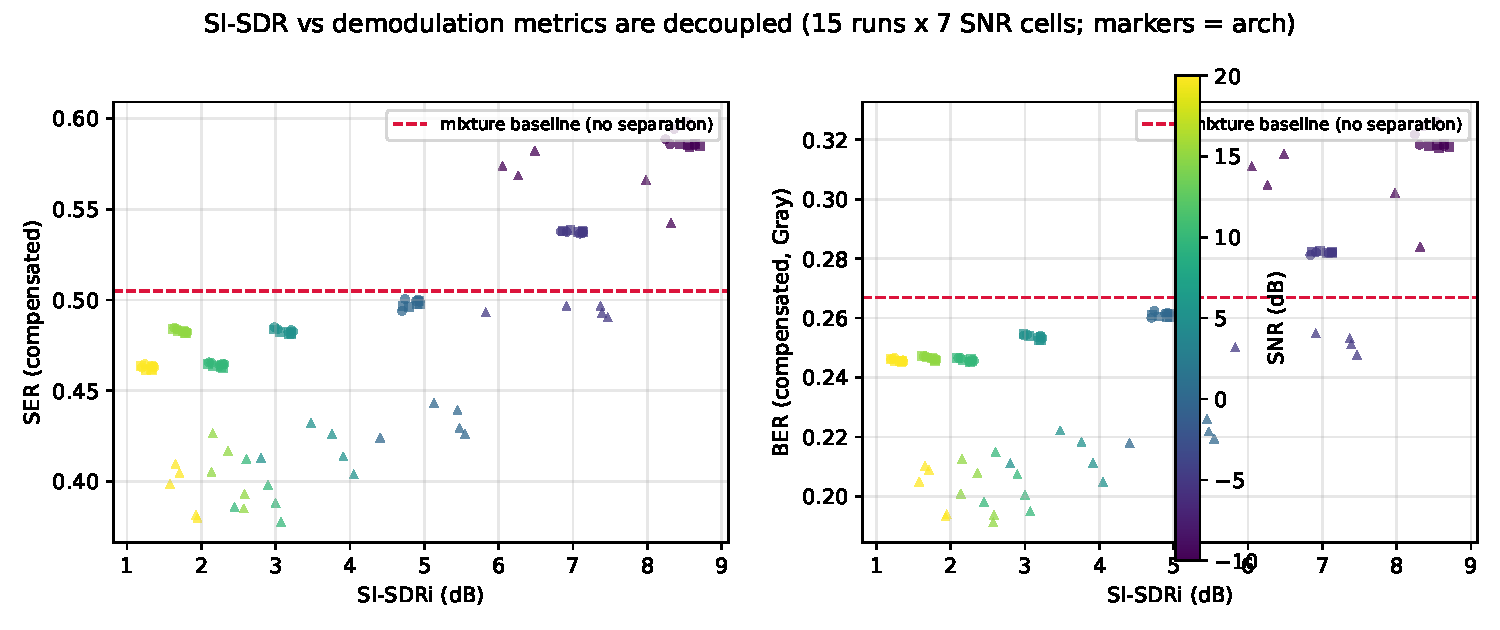
\includegraphics[width=0.95\columnwidth]{figures/s1_sisdr_vs_ser_ber.pdf}
\caption{S1: SI-SDR improvement is decoupled from demodulation. Each
marker is a (run $\times$ SNR) cell of fifteen variable-$K$ separators
(three architectures, five seeds; markers = architecture, colour =
SNR); the dashed line is the unseparated-mixture baseline. SER (left)
and Gray BER (right) stay on the baseline across a 1--9\,dB SI-SDRi
range. The recursive architecture's sub-baseline triangle cells are a
selection-bias artefact (its 37\,\% miss rate restricts scoring to
matched pairs); the honest slot/specialist cells sit on the baseline.}
\label{fig:s1scatter}
\end{figure}

\begin{figure}[!t]
\centering
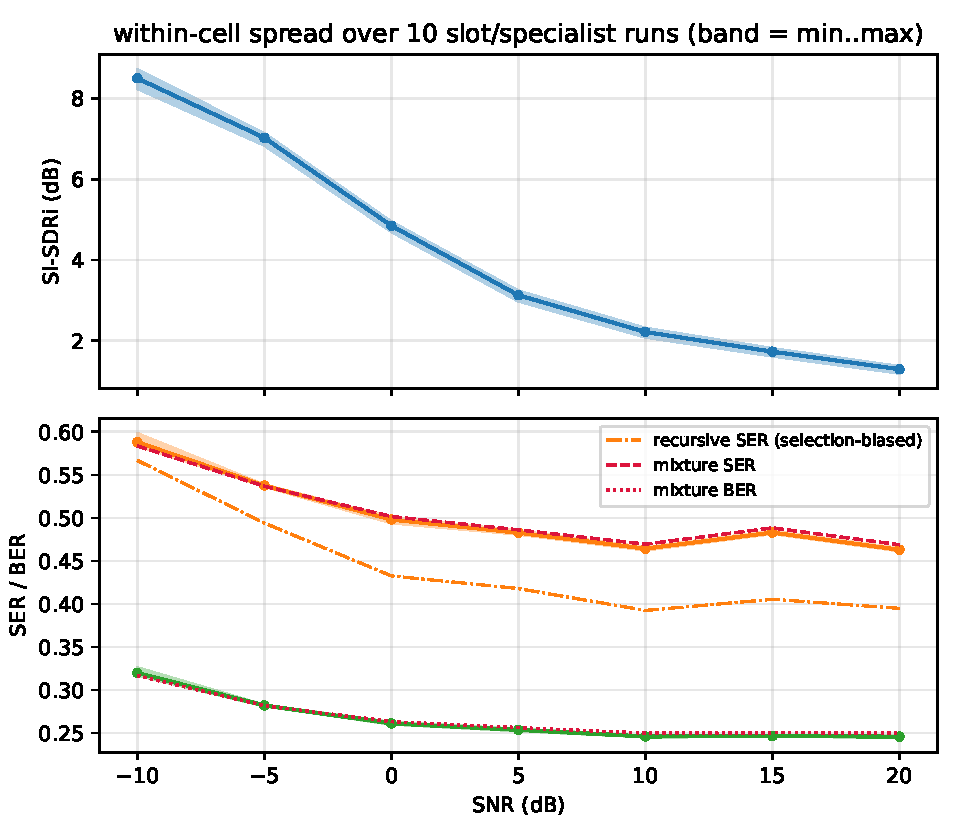
\includegraphics[width=0.7\columnwidth]{figures/s1_flat_region.pdf}
\caption{S1: the flat region, per SNR. Top: SI-SDRi of the
slot/specialist runs (band = min..max over ten runs). Bottom:
compensated SER/BER of the same runs against the mixture baselines
(dashed/dotted); the recursive architecture (dash-dot) is shown
separately because its miss rate biases its SER downward. Waveform
quality improves by 2--8\,dB across the grid while bit-level metrics
do not move.}
\label{fig:s1flat}
\end{figure}

One apparent exception is worth naming precisely because it is an
artefact: the recursive architecture's SER of $0.4477 \pm 0.0063$
\emph{looks} better than the baseline, but its 37\,\% miss rate means
SER is computed only on source pairs it managed to separate---a
selection-biased subset. A matched-pair control settles this directly:
on exactly the source pairs the recursive model matched, the
unprocessed mixture itself scores $0.4454 \pm 0.0062$---
statistically indistinguishable from the model's own $0.4477$ (the
model is, if anything, $0.002$ \emph{worse} on its own matched subset,
and the two track each other at every SNR). The apparent $+5.7$\,pp
gain over the full-cohort baseline is entirely the selection effect, so
the number is excluded from the comparison
(it is retained in the figures, flagged, for transparency). The honest
reading of S1 is that \emph{SI-SDR-optimal separation is BER-blind at
$\sir \approx 0$\,dB}: the residual that remains after separation is
co-channel interference leakage comparable in power to the target
symbol itself---several times the decision half-distance of even the
densest constellation---and waveform polishing within this model class
has so far not crossed the decision boundaries.

\emph{An SIR sweep at fixed $K{=}2$.} The flatness could in principle
be specific to the symmetric point $\sir \approx 0$\,dB, so we
re-evaluate the slot checkpoints (config (b), five seeds) on
fixed-$K{=}2$ test sets whose mixing weights are set to
$\sir \in \{0, 5, 10, 20\}$\,dB (geometrically symmetric about the
training mean $0.5$; independent test seed 88888), keeping the full
SNR grid (Table~\ref{tab:sir_sweep}). The pooled SER \emph{does} fall
with SIR ($0.563 \to 0.466$)---but so does the per-cell mixture
baseline ($0.571 \to 0.457$), and the gap between the two never exceeds
one percentage point, crosses zero near $\sir = 10$\,dB and turns
clearly negative at $20$\,dB, while the
SI-SDRi holds at $+3.0$ to $+3.9$\,dB throughout. The SIR-driven
improvement is entirely the strong source's (SER $0.43 \to 0.19$ as
its interferer fades) while the weak source degrades
($0.67 \to 0.74$): asymmetric SIR does not make the \emph{pair} more
separable in bits---it merely re-weights the cell toward the source
that needed no separation. The waveform--bit mismatch is therefore not
a property of the symmetric point; it persists across the swept range.
(Caveat: training used $\sir \approx 0$\,dB, so the
$\sir > 3.5$\,dB cells are out-of-distribution; the held SI-SDRi shows
the separator still functions there. An SIR-matched training sweep is
future work.)

\begin{table}[H]
\centering
\caption{SIR sweep at fixed $K{=}2$ (mixing weights set to geometrically symmetric SIR levels about the training mean; independent test seed 88888, full SNR grid; config (b), 5 seeds). $\Delta$ is baseline $-$ model in percentage points. The pooled SER falls with SIR, but so does the per-cell mixture baseline, and the gap never exceeds one point (crossing zero near $10$\,dB, clearly negative at $20$\,dB) while SI-SDRi holds --- the improvement is entirely the strong source's (SER $0.43 \to 0.19$) as its interferer fades; the weak source degrades ($0.67 \to 0.74$). The waveform--bit mismatch is not specific to $\sir \approx 0$\,dB. Models are trained at $\sir \approx 0$\,dB, so the $\sir > 3.5$\,dB rows are out-of-distribution.}
\label{tab:sir_sweep}
\setlength{\tabcolsep}{4pt}
\footnotesize
\begin{tabular}{r r r r r r}
\toprule
SIR (dB) & Baseline SER & (b) SER & $\Delta$ (pp) & SI-SDRi (dB) & SER strong / weak \\
\midrule
0 & 0.5710 & 0.5629 $\pm$ 0.0016 & $+0.82$ & +3.2 & -- / -- \\
5 & 0.5500 & 0.5478 $\pm$ 0.0006 & $+0.22$ & +3.6 & 0.426 / 0.669 \\
10 & 0.4921 & 0.4923 $\pm$ 0.0002 & $-0.02$ & +3.9 & 0.273 / 0.712 \\
20 & 0.4569 & 0.4658 $\pm$ 0.0033 & $-0.89$ & +3.0 & 0.193 / 0.738 \\
\bottomrule
\end{tabular}
\end{table}


\subsection{S2: Task-oriented training}
\label{sec:s2}

Table~\ref{tab:s2_main} is the main matrix: five loss configurations of
Eq.~\eqref{eq:loss}, five seeds each, evaluated by the compensated
receiver. Fig.~\ref{fig:s2pareto} shows the same numbers in the
SI-SDRi$\,\times\,$SER/BER plane. Four readings, in decreasing order of
what a reader might hope for.

\begin{table}[H]
\centering
\caption{S2 main matrix (slot architecture, $K\in\{1,2,3\}$, 5 seeds except where noted; mean $\pm$ population std across seeds). The soft-demodulation loss has at most a practically negligible effect on bit-level metrics. Seed-level exact paired permutation tests ($n{=}5$, two-sided; smallest attainable $p{=}2/2^5{=}0.0625$, power-limited) give (c) ser vs.\ (a) SI-SDR, BER: $\Delta{=}+0.0008$, $p{=}0.1875$; (c) ser vs.\ (b) MSE, BER: $\Delta{=}+0.0013$, $p{=}0.1250$; (d) ser+mse vs.\ (a) SI-SDR, SER: $\Delta{=}-0.0012$, $p{=}0.1875$. A cell-level test (7 SNR $\times$ 5 seeds $=$ 35 paired differences, $10^6$ Monte-Carlo sign-flips) returns small $p$-values for config (c) ((c) vs.\ (a), BER: $\Delta{=}+0.00102$, $p{=}0.0004$; (c) vs.\ (b), BER: $\Delta{=}+0.00169$, $p{=}0.0001$, nominally surviving a Bonferroni $\alpha{=}0.05/8{=}0.00625$ over the 8 contrasts. The effect is concentrated in the high-SNR cells ($15$--$20$\,dB, $+0.2$--$0.3$\,pp in the cell means; 4/5 seeds agree in sign, seed-level $p{=}0.125$ power-capped) and vanishes at low SNR; the fair additive comparison (d) vs.\ (b) shows nothing (SER $p{=}0.38$, BER $p{=}0.61$), nor does any SER contrast) --- but it treats within-seed cells as exchangeable even though they share one trained model, so it is anti-conservative and is reported as descriptive only; the defensible summary at $n{=}5$ is $|\Delta| \le 0.17$\,pp with an unstable sign. Config (c) replaces the MSE anchor with the soft-SER term; the additive design is (d). The soft-SER term does improve source counting (count acc.\ $0.65\!\rightarrow\!0.85$, occupancy route) and suppresses hallucinated sources. Configs (a)--(e) as defined in Section~\ref{sec:configs}. $^{\dagger}$single seed ($n{=}1$), no std.}
\label{tab:s2_main}
\setlength{\tabcolsep}{2pt}
\scriptsize
\begin{tabular}{l r r r r r}
\toprule
Config & SI-SDRi (dB) & SER & BER & Count acc. & Halluc. \\
\midrule
(a) SI-SDR & +4.23 $\pm$ 0.02 & 0.5022 $\pm$ 0.0002 & 0.2646 $\pm$ 0.0001 & 0.649 $\pm$ 0.018 & 0.155 $\pm$ 0.009 \\
(b) MSE & +4.07 $\pm$ 0.10 & 0.5027 $\pm$ 0.0007 & 0.2651 $\pm$ 0.0005 & 0.658 $\pm$ 0.023 & 0.149 $\pm$ 0.015 \\
(c) soft-SER & +3.91 $\pm$ 0.02 & 0.5031 $\pm$ 0.0017 & 0.2638 $\pm$ 0.0009 & 0.850 $\pm$ 0.088 & 0.060 $\pm$ 0.035 \\
(d) soft-SER + MSE & +3.72 $\pm$ 0.10 & 0.5034 $\pm$ 0.0013 & 0.2647 $\pm$ 0.0011 & 0.857 $\pm$ 0.032 & 0.049 $\pm$ 0.017 \\
(e) pure soft-SER & -9.42$^{\dagger}$ & 0.5159$^{\dagger}$ & 0.2713$^{\dagger}$ & 0.913$^{\dagger}$ & 0.034$^{\dagger}$ \\
Mixture (no separation) & -- & 0.5049 & 0.2669 & -- & -- \\
\bottomrule
\end{tabular}
\end{table}


\begin{figure}[!t]
\centering
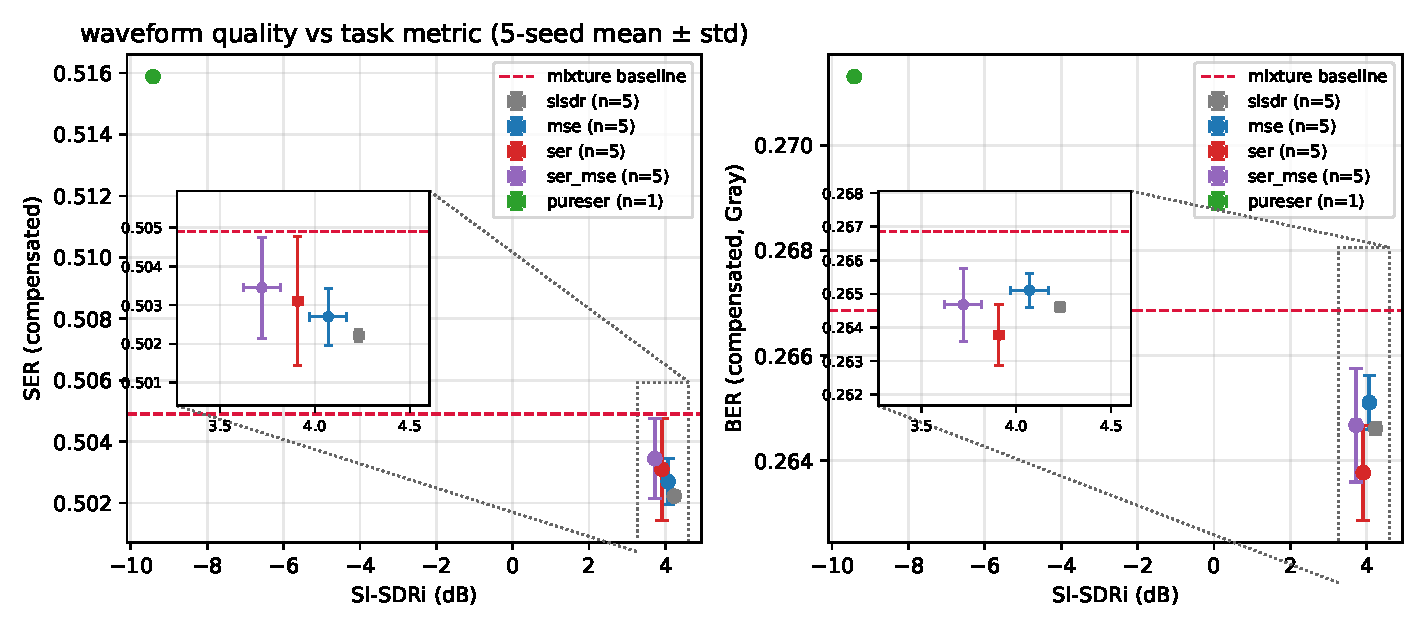
\includegraphics[width=0.95\columnwidth]{figures/s2_pareto.pdf}
\caption{S2: waveform quality vs.\ task metrics (5-seed mean $\pm$
population std). Configs (a)--(d) cluster within 0.5\,dB SI-SDRi and
$0.001$ SER of each other, all on the mixture baseline (dashed); the
pure task loss (e) collapses off the manifold (left edge).}
\label{fig:s2pareto}
\end{figure}

\emph{1. Pooled bit-level effect: practically negligible, and not
statistically resolvable at $n{=}5$ seeds.} The seed-level exact
test---the cluster-correct one, since the seven SNR cells of a seed
share a single trained model---is power-capped ($p \geq 0.0625$
attainable) and finds nothing: (c) vs.\
(a) BER $\Delta = +0.0008$, $p = 0.1875$; (c) vs.\ (b) BER
$\Delta = +0.0013$, $p = 0.1250$; (d) vs.\ (a) SER
$\Delta = -0.0012$, $p = 0.1875$. The cell-level test pools 35
(seed $\times$ SNR) differences and does return small $p$-values for
config (c)---BER $\Delta = +0.00102$ vs.\ (a)
($p = 0.0004$) and $\Delta = +0.00169$ vs.\ (b) ($p = 0.0001$), both
surviving Bonferroni over the eight contrasts, concentrated in the
high-SNR cells (15/20\,dB: $+0.2$--$0.3$\,pp in the cell means, 4/5 seeds
agree in sign)---but its sign-flips treat within-seed cells as
exchangeable, which they are not; the test is anti-conservative here
and we report it only as descriptive. The defensible summary at
$n{=}5$ is $|\Delta| \leq 0.17$\,pp with an unstable sign, not a
demonstrated effect. But (c)
\emph{replaces} the MSE anchor (Section~\ref{sec:configs}), so these
numbers confound the task term with the anchor's removal; the fair
additive comparison is (d) vs.\ (b), which buys at most $\sim$0.03\,pp
(BER $\Delta = +0.00027$, $p = 0.61$) and is null on SER ($p = 0.38$).
One marginal contrast deserves disclosure: (d) vs.\ (a) SER has
cell-level $\Delta = -0.00173$ with permutation $p = 0.064$---non-significant under
our primary test---yet a paired-bootstrap 95\,\% CI of
$[-0.00377, -0.00005]$ grazing zero on the unfavourable side. Percentile
bootstrap CIs are anti-conservative at $n{=}5$ (this is why the
permutation test is primary here), and the per-$K$ decomposition below
shows where this negative tail comes from.

\emph{2. The pool hides a sign flip along the interference axis.}
Table~\ref{tab:s2_perk} decomposes the four contrasts by source count
(seed-level exact permutation per $K$). At $K{=}1$---no interference,
receiver-limited---the contrasts are small and sign-unstable
($-0.01$/$-0.19$/$+0.26$/$+0.45$\,pp BER across the four contrasts; at
best 4/5 seeds agree, and the largest value is driven mostly by a
single seed). At $K{=}2$, the $\sir \approx 0$\,dB case that motivates
task-oriented training, the term \emph{helps}, consistently: BER
$+0.35$\,pp (c vs.\ a) / $+0.40$\,pp (c vs.\ b) and
$+0.11$\,pp / $+0.06$\,pp in the fair additive contrasts (d vs.\ b /
d vs.\ a), with 5/5 seeds
positive in \emph{all four} contrasts (exact $p = 0.0625$, the $n{=}5$
floor). At $K{=}3$ the sign reverses: SER $-0.60$ to $-0.72$\,pp with
0/5 seeds positive in \emph{all four} contrasts ($p = 0.0625$). Weighted
by the 1:2:3 pair counts, the $K{=}2$ gain and the $K{=}3$ loss cancel
into the pooled $\leq 0.17$\,pp of Table~\ref{tab:s2_main}. The number
of interferers is a more incisive experimental variable than the SNR
proxy of reading~1: same loss, same backbone, same SNR grid---and the
sign of the bit-level effect flips with the interference order. The
negative tail of the (d) vs.\ (a) SER contrast above is precisely the
$K{=}3$ effect.

\begin{table}[H]
\centering
\caption{S2 per-$K$ decomposition of the four pre-declared contrasts (5 paired seeds per cell; exact two-sided sign-flip permutation, $2^5{=}32$). Cells give the mean paired difference in \textbf{percentage points} (positive favours the first-named configuration) and the number of seeds with a positive difference. Exact $p$: $0.0625$ for $5/5$ or $0/5$ (the $n{=}5$ floor), $0.125$ for $1/5$, $\geq 0.125$ for $4/5$ (the exact value depends on the seed magnitudes), $\geq 0.25$ otherwise. The pooled null of Table~\ref{tab:s2_main} resolves into structure: at $K{=}2$ the soft-SER term helps (BER positive, $5/5$ seeds in \emph{all four} contrasts); at $K{=}3$ it hurts (SER negative, $0/5$ seeds in \emph{all four} contrasts); at $K{=}1$ there is no interference and the contrasts are small and sign-unstable. The two cancel under the 1:2:3 pair-count weighting of the pool.}
\label{tab:s2_perk}
\setlength{\tabcolsep}{4pt}
\footnotesize
\begin{tabular}{ll r r r}
\toprule
Contrast & Metric & $K{=}1$ & $K{=}2$ & $K{=}3$ \\
\midrule
(c) soft-SER vs (a) SI-SDR & SER & $-0.03$ (2/5) & $+0.53$ (4/5) & $-0.72$ (0/5) \\
(c) soft-SER vs (a) SI-SDR & BER & $-0.01$ (3/5) & $+0.35$ (5/5) & $-0.15$ (0/5) \\
\addlinespace[2pt]
(c) soft-SER vs (b) MSE & SER & $-0.44$ (2/5) & $+0.59$ (3/5) & $-0.71$ (0/5) \\
(c) soft-SER vs (b) MSE & BER & $-0.19$ (2/5) & $+0.40$ (5/5) & $-0.14$ (0/5) \\
\addlinespace[2pt]
(d) soft-SER+MSE vs (b) MSE & SER & $+0.53$ (4/5) & $+0.32$ (4/5) & $-0.60$ (0/5) \\
(d) soft-SER+MSE vs (b) MSE & BER & $+0.26$ (4/5) & $+0.11$ (5/5) & $-0.10$ (1/5) \\
\addlinespace[2pt]
(d) soft-SER+MSE vs (a) SI-SDR & SER & $+0.94$ (4/5) & $+0.25$ (4/5) & $-0.61$ (0/5) \\
(d) soft-SER+MSE vs (a) SI-SDR & BER & $+0.45$ (4/5) & $+0.06$ (5/5) & $-0.12$ (1/5) \\
\addlinespace[2pt]
\bottomrule
\end{tabular}
\end{table}


\emph{3. A structural side benefit: occupancy gating, with a caveat.}
The soft-SER term markedly improves the occupancy structure:
occupancy-routed count accuracy rises from $0.649 \pm 0.018$ (a) /
$0.658 \pm 0.023$ (b) to $0.850 \pm 0.088$ (c) / $0.857 \pm 0.032$ (d),
and the hallucination rate falls from $\sim$0.15 to $0.05$--$0.06$; the
effect is largest exactly where the occupancy route was broken: its
$K{=}2$ count accuracy rises from a $0.035$ mean (per-seed
$0.001$--$0.11$) to $0.63$ (per-seed $0.19$--$0.84$---the spread is
wide, and one seed barely improves). Two qualifications keep this
benefit honest. First, the occupancy route's tol-1 count accuracy is
already $0.97$--$1.00$ in \emph{all} configurations---it always counts
within one---so the term largely \emph{recalibrates the $K{=}2$
occupancy threshold} rather than conferring counting ability; a
threshold-free gating score would be the cleaner evidence and is future
work. Second, the dedicated count head sits at $\approx$0.9
($0.87$--$0.92$) for all
configurations and still beats the repaired occupancy route, so the
task term does not produce the best $K$ estimate. The defence: the
occupancy probabilities \emph{gate the slot outputs}---they decide
which waveforms are passed to the downstream receiver---and
hallucinated slots are output waveforms, not just a wrong count.
Halving hallucinated outputs is a bit-stream-relevant improvement that
the count-head number does not capture.

\emph{4. The waveform objective is load-bearing.} Config (e), the pure
task loss, reaches SER 0.5159---\emph{worse than the unseparated
mixture}---with SI-SDRi $-9.42$\,dB, while its training soft-SER
decreases normally (2.24 $\to$ 1.81): the optimiser found waveforms
that minimise the soft receiver's cross-entropy without separating, an
off-manifold reward hack. The proxy--truth parity verified on clean
sources (Section~\ref{sec:loss}) holds only near the clean manifold;
far from it, proxy and truth decouple, and only the waveform terms
confine the model to the manifold. Waveform supervision is thus
\emph{necessary but not sufficient}.

\subsection{Ablations: dose, temperature, and what is not happening}
\label{sec:abl}

Table~\ref{tab:s2_ablation} varies the two knobs of the task term
(single seed). Neither shows a dose--response on the task metrics:
across $\lambda_{\mathrm{ser}} \in \{0.3, 1, 3\}$ and
$\sigma^2 \in \{0.05, 0.1, 0.2\}$, compensated SER/BER stay within
$\approx$0.005 of the controls, while $\lambda_{\mathrm{ser}}$
monotonically trades SI-SDRi ($+4.2 \to +2.7$\,dB at
$\lambda_{\mathrm{ser}} = 3$) for occupancy accuracy
($0.68 \to 0.93$) and hallucination suppression ($0.14 \to 0.02$).
The counting benefit is therefore real, monotone, and cheap; the bit
benefit is not purchasable at any dose. Consistently, the training
trajectory of the soft-SER term in config (c) is nearly flat
(2.95 $\to$ 2.84): at $\lambda_{\mathrm{ser}} = 1$ its gradient is
dominated by the waveform terms, yet raising its weight a full order of
magnitude still buys no SER/BER movement---the flatness is not an
optimisation artefact of loss scale.

\begin{table}[H]
\centering
\caption{S2 ablation of the soft-demodulation loss weight $\lambda_{\mathrm{ser}}$ and the soft-decision Gaussian width $\sigma^2$ (single seed 42, slot architecture). Neither knob shows a dose--response on compensated SER/BER --- all values remain within $\approx\!0.005$ of the controls --- while larger $\lambda_{\mathrm{ser}}$ monotonically improves occupancy accuracy and reduces hallucination, at the cost of SI-SDRi. Counting metrics use the occupancy route.}
\label{tab:s2_ablation}
\setlength{\tabcolsep}{3pt}
\footnotesize
\begin{tabular}{l r r r r r r r}
\toprule
Config & $\lambda_{\mathrm{ser}}$ & $\sigma^2$ & SI-SDRi (dB) & SER & BER & Occ.\ acc. & Halluc. \\
\midrule
sisdr (control) & -- & -- & +4.26 & 0.5020 & 0.2644 & 0.684 & 0.139 \\
ser (control) & 1 & 0.1 & +3.90 & 0.5018 & 0.2631 & 0.912 & 0.040 \\
ser, $\lambda_{\mathrm{ser}}{=}0.3$ & 0.3 & 0.1 & +4.19 & 0.5029 & 0.2643 & 0.768 & 0.105 \\
ser, $\lambda_{\mathrm{ser}}{=}3.0$ & 3 & 0.1 & +2.67 & 0.5046 & 0.2647 & 0.932 & 0.023 \\
ser, $\sigma^2{=}0.05$ & 1 & 0.05 & +3.16 & 0.5054 & 0.2655 & 0.922 & 0.028 \\
ser, $\sigma^2{=}0.2$ & 1 & 0.2 & +4.13 & 0.5033 & 0.2644 & 0.831 & 0.077 \\
\bottomrule
\end{tabular}
\end{table}


Two negative checks complete the picture. \emph{No implicit
equalisation}: config (c)'s per-modulation SER (0.236, 0.412, 0.620,
0.742 for BPSK, QPSK, 8PSK, 16QAM) remains far from the clean-source
floors (0.000, 0.000, 0.014, 0.032), so the task loss did not learn to
invert the multipath channel, even implicitly. \emph{No hidden capacity issue}:
the counting gains show the term's gradients do reach and reshape the
backbone---the bottleneck is not gradient flow but the interference
structure itself.

\subsection{S3: Joint soft-information detection---a diagnosed negative result}
\label{sec:s3}

S3 tests the strongest task-oriented design: bypass the explicit
waveform and read per-source symbol posteriors off the joint
representation (Section~\ref{sec:jointhead}), at fixed $K{=}2$ where the
SIR$\,\approx\,$0 pressure is real but the count is known.
Table~\ref{tab:s3} and Fig.~\ref{fig:s3bars} give the outcome: both head
versions sit at the modulation-averaged chance level (SER
$\approx 0.73$ vs.\ chance 0.766; BER $\approx 0.46$ vs.\ random-bit
0.500), far \emph{worse} than the unseparated mixture (0.5612/0.2872)
and than the same model's own waveform route through the compensated
receiver (0.5437/0.2758, which stays intact---SI-SDRi($K{=}2$)
$+3.46$\,dB). The remaining row anchors this cross-study: the S2
task-loss model's waveform route on the same $K{=}2$ cell
(0.5475/0.2777) sits within one std of S3's own waveform route, so the
backbone operates at its expected level when the head fails. Paired
bootstrap differences are decisive ($\Delta$SER
$+0.1860$, 95\,\% CI $[+0.1805, +0.1915]$ for v2 vs.\ the waveform
route). The classical ``joint detection beats separate-then-detect''
does \emph{not} come for free by attaching a head.

\begin{table}[H]
\centering
\caption{S3 joint LLR head vs.\ waveform routing, $K{=}2$ cell (5 seeds, mean $\pm$ std; baseline is single-pass). The joint head is significantly WORSE than every reference: paired bootstrap gives $\Delta$SER ${=}+0.1860$ (95\% CI $[+0.1805, +0.1915]$) for v2 vs.\ the S3 waveform route and $\Delta$SER ${=}+0.1685$ ($[+0.1670, +0.1701]$) vs.\ the mixture baseline --- all CIs far from 0 (v1: $\Delta$SER ${=}+0.1857$ vs.\ waveform). Both variants sit at the modulation-averaged chance level (SER $\approx 0.73$, BER $\approx 0.46$). Candidate failure causes: v1's boxcar averaging cancels the nominal $2000$\,Hz carrier almost exactly (inferred from the architecture, not verified on features); v2's learned strided convolutions cannot recover burst-level carrier/phase blindly --- a controlled $K{=}1$ probe with oracle sync trains the same head to val SER $0.15$ vs.\ $0.68$ under blind sync, but at $K{=}2$ even a frequency-oracle probe (per-source phase alignment is impossible for a mixture) reaches only $0.589$, worse than the mixture baseline ($0.561$): synchronisation alone is not sufficient under phase entanglement.}
\label{tab:s3}
\setlength{\tabcolsep}{4pt}
\footnotesize
\begin{tabular}{l r r}
\toprule
Route ($K{=}2$) & SER & BER (Gray) \\
\midrule
Mixture (no separation) & 0.5612 & 0.2872 \\
S2-ser waveform route & 0.5475 $\pm$ 0.0063 & 0.2777 $\pm$ 0.0031 \\
S3 waveform route (v2 model) & 0.5437 $\pm$ 0.0083 & 0.2758 $\pm$ 0.0056 \\
S3 joint head v1 (window mean) & 0.7324 $\pm$ 0.0021 & 0.4668 $\pm$ 0.0015 \\
S3 joint head v2 (learned strided conv) & 0.7297 $\pm$ 0.0018 & 0.4639 $\pm$ 0.0011 \\
\bottomrule
\end{tabular}
\end{table}


\begin{figure}[!t]
\centering
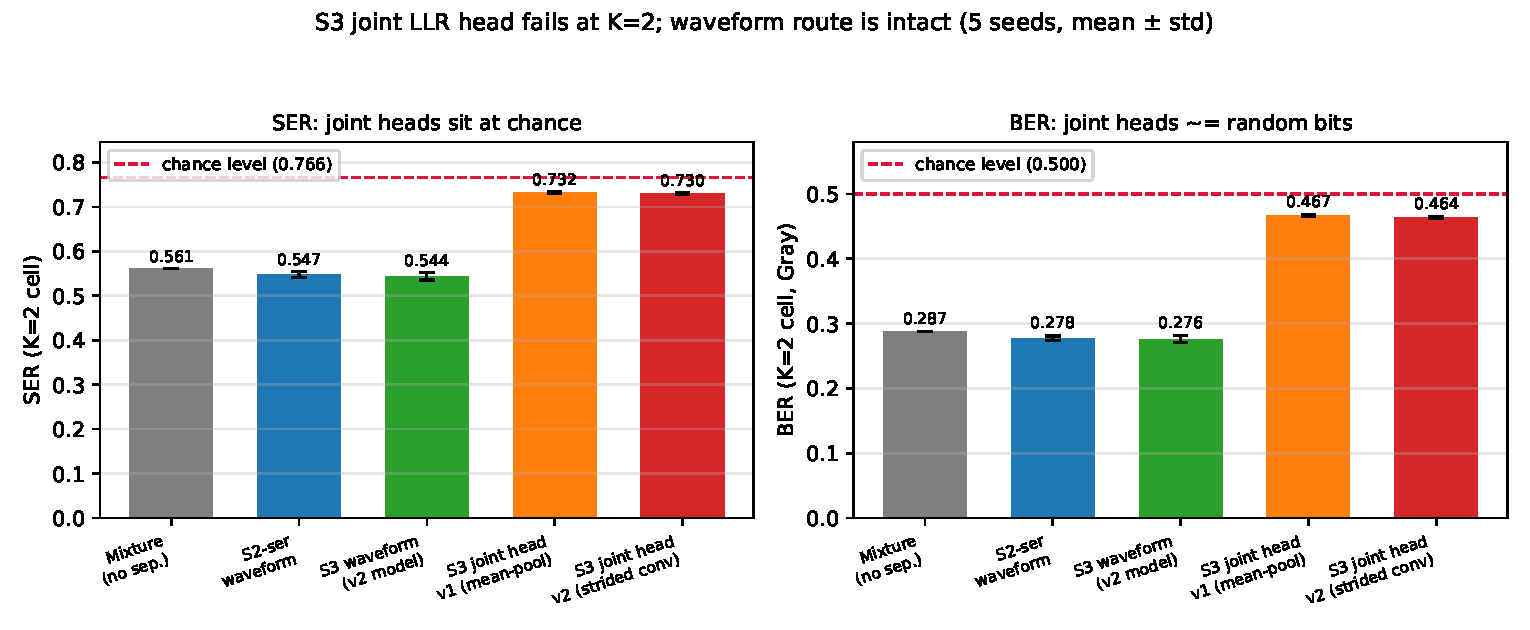
\includegraphics[width=0.95\columnwidth]{figures/s3_joint_vs_waveform.pdf}
\caption{S3 ($K{=}2$ cell, 5 seeds): joint-head routes (orange/red) sit
at chance (dashed), while the waveform route through the compensated
receiver (green) is intact. The failure is in the head's front-end, not
in the shared backbone.}
\label{fig:s3bars}
\end{figure}

The failure is informative because it has two separately identified
causes. \emph{v1 (window mean)}: the fixed 16-sample boxcar averages
two full cycles of the nominal 2000\,Hz carrier at $f_s = 16$\,kHz, so
on a passband waveform its mean cancels almost exactly---the true
carriers wander within $-5$/$+10$\,Hz of the nominal value, so the
cancellation is exact only at 2000\,Hz; v1's head consumes
\emph{learned features} rather than the raw waveform, so carrier
starvation is inferred---from the architecture and from a training
plateau in which joint 16QAM SER sits at $\approx 0.92 \approx$
chance---rather than directly verified on the features themselves.
We therefore treat the window-mean trap as a candidate cause, not the
established one. \emph{v2 (learned strided conv)}:
replacing the trap changes nothing (0.7297 vs.\ 0.7324)---granted, the
replacement's 32-tap kernel is itself shorter than the 65-tap matched
filter, so the replacement is only a partial fix---because the
deeper obstacle remains: each source still carries an arbitrary burst
phase and residual frequency offset that the evaluation receiver removes
with oracle knowledge and a 256-symbol phase fit, while the symbol-rate
head's receptive field spans only $\pm 4$ symbols. A controlled probe
supports this attribution: the \emph{same} head architecture, on $K{=}1$
data with no separation and no PIT, plateaus at val SER 0.68 ($\approx$
chance) when it must synchronise blindly, but reaches 0.150 and is still
improving when given oracle down-conversion and burst-level phase
alignment (Fig.~\ref{fig:s3probe}; per-modulation: BPSK 0.03, QPSK 0.09,
8PSK 0.25, 16QAM 0.24 vs.\ 0.38/0.68/0.85/0.81 blind). Note what the
probe does \emph{not} show: even with oracle synchronisation the head's
0.150 merely matches the $K{=}1$ waveform-route baseline (0.146)---the
probe establishes blind synchronisation as a \emph{necessary}
explanation of the failure, not that fixing it would be
\emph{sufficient}. We read this as
pointing to burst-level blind carrier/phase recovery as the binding
constraint for neural joint detection in this setting; the probe is
$K{=}1$ while the head fails at $K{=}2$, so we also run the $K{=}2$
version of the same probe (\texttt{probe\_sync\_head\_k2.py}).

At $K{=}2$ the oracle can only be partial: down-converting the mixture
at each source's true carrier removes the frequency search (two oracle
channels), but per-source phase alignment is impossible in
principle---the two sources' phases are entangled in the single
observed mixture. With this frequency oracle the two-slot probe head
reaches val SER $0.589$, \emph{worse} than the unseparated-mixture
baseline ($0.561$) and far worse than the waveform route through the
separator ($0.5475$); the blind variant stalls at $0.711$. The $K{=}1$
rescue therefore does not transfer: at $K{=}2$ the binding constraint
is not the frequency search but joint detection under phase
entanglement---precisely the structure that classical multiuser
detection makes explicit~\cite{verdu1998multiuser,dankberg1998pcma}.

\begin{figure}[!t]
\centering
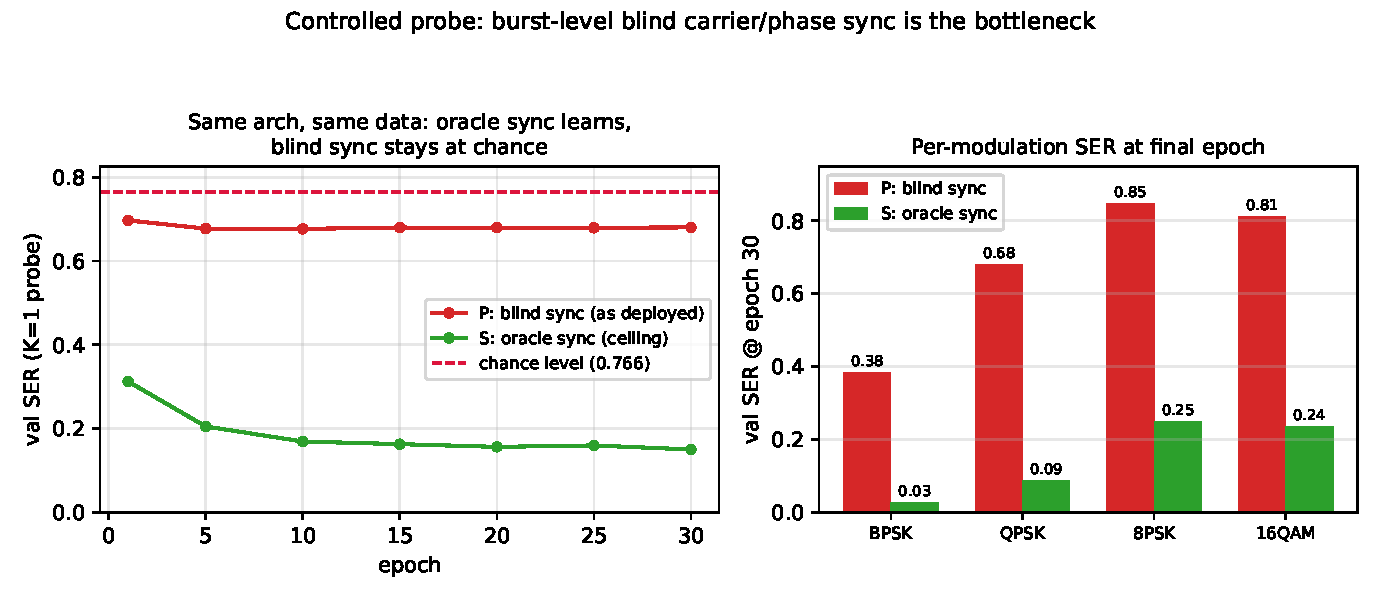
\includegraphics[width=0.95\columnwidth]{figures/s3_probe_sync.pdf}
\caption{Controlled synchronisation probe ($K{=}1$, no separation): the
same head learns with oracle synchronisation (green, val SER
0.31$\to$0.15) and stalls at chance when synchronising blindly (red).
Left: learning curves; right: per-modulation SER at the final epoch.}
\label{fig:s3probe}
\end{figure}

% ======================================================================
\section{Discussion}
\label{sec:disc}

\emph{What the task loss can and cannot buy.} The soft-SER term and the
SI-SDR term are different metrics, but they attack overlapping feasible
sets. SI-SDR is invariant to scale and to a global phase rotation, and
the oracle-synchronised soft receiver removes exactly those two
receiver-side nuisances (unit-power grid, phase-only alignment)---no
more. It performs no timing search and no equalisation, so timing- and
ISI-shaped errors lie outside the reach of \emph{both} objectives
(SI-SDR is in any case shift-sensitive, and Section~\ref{sec:abl}
confirms that no implicit equalisation emerged). What the soft term adds
over the waveform loss is therefore not a new degree of freedom but new
\emph{information}: where the residual mass sits relative to the
constellation's decision boundaries. The per-$K$ decomposition prices
that information, and it is the interference order that sets the price.
At $K{=}1$ the residual is noise and multipath ISI; boundary information
buys nothing. At $K{=}2$ a single leaked interferer leaves recoverable
structure---borderline symbols sit close enough to a boundary that a
grid-aware gradient nudges a reproducible fraction of them across
($+0.35$\,pp BER, 5/5 seeds). At $K{=}3$ the same gradient turns
misleading: with two interferers leaking, the residual cloud contains
the \emph{other} sources' modulated mass as well as the target's, and
pulling estimates toward the nearest constellation points can pull them
toward the wrong constellation ($-0.6$ to $-0.7$\,pp SER, 0/5 seeds).
We flag this $K{=}3$ account as a hypothesis fitted to the observed
sign pattern; the sign pattern itself---and its cancellation in the
pool---is the robust observation. Two mundane alternatives are not
excluded: the loss averages the soft-SER term over a sample's sources,
so a $K{=}3$ sample receives one third of the per-source task gradient
of a $K{=}1$ sample (gradient dilution rather than misdirection), and
at $\sigma^2 = 0.1$ on the unit-power grid the soft receiver's logits
saturate---16QAM's nearest-neighbour distance already gives
$d^2/\sigma^2 \approx 4$, and typical residuals sit much further
off-grid---which by itself would explain both the flat soft-SER
training trajectory ($2.95 \to 2.84$) and the flat dose--response; the
$\sigma^2$ ablation reached only 0.2, still inside the saturated
regime. A per-$K$ dose--response at larger $\sigma^2$ would separate
these accounts. All effects stay in the
fraction-of-a-point range because at $\sir \approx 0$\,dB the leakage
power is comparable to the target symbol's own (several times the 0.32
decision half-distance of 16QAM on the unit-power grid): no loss
reweighting changes the interference order. The dose--response ablation
(Section~\ref{sec:abl}) closes the alternative explanation that the term
was simply under-weighted, and the additive (d) vs.\ (b) reading caps
the deployable gain at $\sim$0.03\,pp.

\emph{What the soft receiver sees and what it does not.} The reward hack
of config (e) shows the proxy--truth alignment is a local guarantee: on
or near the clean manifold the differentiable receiver \emph{is} the
evaluation receiver (symbol-for-symbol parity), but nothing prevents the
optimiser from leaving that manifold when the waveform anchor is
removed, and off-manifold the proxy can be minimised while true SER
worsens. Task losses, like adversarially trained discriminators, need
the generator pinned to the data manifold; here the waveform terms play
that role.

\emph{Why counting improves.} The occupancy head's errors are leakage
errors: residual energy of a true source bleeding into a nominally empty
slot (hallucination) or a true slot failing to concentrate its source
(missed occupancy, e.g.\ the $K{=}2$ collapse to a $0.035$ mean under
waveform losses). A demodulation-shaped penalty is sensitive to exactly this
energy's \emph{position relative to decision boundaries}, not merely its
total power, and it reaches the occupancy head through the shared
backbone. The result---occupancy-routed counting repaired from $0.65$ to
$0.85$ (from near-chance at $K{=}2$) without touching the count
loss---suggests task-shaped terms as
general regularisers for structured prediction heads, even where they
cannot improve the task metric itself.

\emph{Consequences for system design.} Three of our results point the
same way. S1: waveform gains do not reach the bits at SIR$\,\approx\,$0
---nor anywhere in an SIR sweep up to $20$\,dB, where the gain over the
per-cell baseline never exceeds one point. S2: loss-level task terms
buy a small, sign-unstable effect whose
direction is dictated by the interference order---helpful against one
interferer, harmful against two---not a dependable gain. S3: folding
detection into the
network fails at the synchronisation step that classical receivers solve
explicitly and our evaluation oracle assumes away---and at $K{=}2$ even
a frequency oracle does not rescue the head (0.589 vs.\ the 0.561
mixture baseline), so what is missing is not sync alone but joint
detection under phase entanglement. Together they say the
binding constraint is \emph{algorithmic structure}, not objective
tuning: explicit burst-level synchronisation and equalisation
(carrier/phase tracking, timing recovery, ISI inversion) inside or
alongside the separator, coupled with explicit joint or successive
multiuser detection---or permutation-invariant training directly on
multiuser-detection likelihoods with synchronisation built in. The
benchmark, the compensated receiver, and the parity-verified soft
receiver released with this paper provide the measurement infrastructure
for exactly that next step.

% ======================================================================
\section{Limitations}
\label{sec:limit}

First and most important: the compensated receiver (and hence the
training loss) uses \emph{oracle} carrier synchronisation and a
burst-level phase fit. This is a deliberate upper-bound truth---it
isolates waveform fidelity from synchronisation---and S3's probe shows
the oracle is doing real work that a deployed blind receiver would have
to do itself; our SER/BER numbers are therefore optimistic as absolute
values, though all \emph{comparisons} share the same oracle. Second,
all signals are synthetic (RRC pulses, three-tap multipath, AWGN); the
interference-limited mechanism should transfer, but the absolute numbers
need not. Third, the variable-$K$ range is $K \leq 3$ (trained) and the
joint head was studied at fixed $K{=}2$ only. Fourth, the reference
labels carry the channel's multipath-ISI floors (up to 3.2\,\% on
16QAM), a label noise shared by all configurations. Fifth, the
cell-level permutation test assumes exchangeable within-seed cell
differences, which does not hold (the seven cells of a seed share one
trained model); we treat it as descriptive only and rely on the
power-capped seed-level test throughout. Sixth, \emph{training} used $\sir \approx 0$\,dB throughout (source
weights $\sim U(0.4, 0.6)$): the evaluation-time SIR sweep of
Section~\ref{sec:s1} extends the picture to $\sir \leq 20$\,dB, but
cells beyond $\sir > 3.5$\,dB are out-of-distribution for these
checkpoints, and an SIR-matched \emph{training} sweep remains future
work. Seventh, the $-10$\,dB SNR test cell lies below the training
range ($[-5, 20]$\,dB), so the $+8.4$\,dB SI-SDRi there is attained at
an extrapolated operating point; we use it only as the largest-gain
cell and no pooled claim depends on it. Eighth, the $K{=}2$
synchronisation probe uses a frequency-only
oracle (per-source phase alignment is impossible for a mixture) and
the same small probe head trained for 30 epochs; a larger head or
longer training might narrow the 0.589 vs.\ 0.561 gap, though the
learning curve has flattened. Finally, config (e) and the ablations
are single-seed probes, used only where marked.

% ======================================================================
\section{Conclusion}
\label{sec:concl}

We have presented, to our knowledge, the first controlled study of the
waveform-to-bit pipeline in single-channel blind separation of
co-frequency communication signals. On a variable-count benchmark with
an offset-compensated receiver as evaluation truth, SI-SDR improvements
of $+4$\,dB---up to $+8.4$\,dB at $-10$\,dB SNR---leave SER/BER on the
unseparated-mixture baseline (a fraction-of-a-point penalty, if
anything, at the lowest SNR), and the flatness persists across an SIR
sweep to $20$\,dB at fixed $K{=}2$ (S1). A differentiable soft-demodulation
loss, verified decision-identical to the evaluation receiver, has a
pooled effect that is practically negligible and not statistically
resolvable at five seeds
($\leq 0.17$\,pp BER; $\leq 0.03$\,pp in the fair additive comparison);
per source count, it helps consistently at $K{=}2$ and hurts
consistently at $K{=}3$, cancelling in the pool (S2). The same term
repairs occupancy gating (count accuracy $0.65 \to 0.85$, hallucination
$0.15 \to 0.05$) and, deprived of the waveform anchor, collapses into
reward hacking---waveform supervision is necessary but not sufficient.
Folding demodulation into a joint head fails at chance; a controlled
probe assigns the cause to burst-level blind synchronisation at $K{=}1$,
while at $K{=}2$ even a frequency oracle fails to beat the mixture
baseline---synchronisation is necessary but not sufficient under
phase-entangled interference (S3). The
practically useful reading: bit-level gains
are \emph{interference-limited, not loss-limited}---progress requires
explicit synchronisation, equalisation, and joint-detection structure,
evaluated at the bit level with the protocol released here.

% ======================================================================
\section*{CRediT authorship contribution statement}
\textbf{Bin Nong:} Conceptualization, Methodology, Software, Validation,
Formal analysis, Investigation, Data curation, Writing -- original
draft, Visualization.
\textbf{Weihong Fu:} Supervision, Project administration, Writing --
review \& editing.
\textbf{Zhuoyun Jiang:} Resources, Validation, Writing -- review \&
editing.

\section*{Declaration of competing interest}
The authors declare that they have no known competing financial
interests or personal relationships that could have appeared to
influence the work reported in this paper.

\section*{Data availability}
Code and synthetic data generators are available at
\url{https://github.com/BinNong/single_channel_source_seperation/tree/main/paper5_task_oriented}.
No external datasets are required.

\section*{Funding}
This research did not receive any specific grant from funding agencies
in the public, commercial, or not-for-profit sectors.

\section*{Declaration of generative AI and AI-assisted technologies in the writing process}
During the preparation of this work the authors used Claude Code
(Anthropic) in order to assist with drafting, editing, and polishing the
manuscript text. After using this tool, the authors reviewed and edited
the content as needed and take full responsibility for the content of
the publication.

% ======================================================================
% Bibliography ordered by first citation (elsarticle numbered style).
\begin{thebibliography}{30}\footnotesize

\bibitem{hou2022single}
X.~Hou and Y.~Gao,
``Single-channel blind separation of co-frequency signals based on
convolutional network,''
\emph{Digital Signal Processing}, vol.~129, p.~103654, 2022,
doi:~\url{https://doi.org/10.1016/j.dsp.2022.103654}.

\bibitem{guo2024single}
P.~Guo, M.~Yu, L.~Shen, Z.~Lin, K.~An, and J.~Wang,
``Single-channel blind source separation in wireless communications: a
complex-domain deep learning approach,''
\emph{IEEE Wireless Commun. Lett.}, vol.~13, no.~6, pp.~1645--1649,
2024, doi:~\url{https://doi.org/10.1109/LWC.2024.3384813}.

\bibitem{kolbaek2017pit}
M.~Kolb{\ae}k, D.~Yu, Z.-H. Tan, and J.~Jensen,
``Multitalker speech separation with utterance-level permutation
invariant training of deep recurrent neural networks,''
\emph{IEEE/ACM Trans. Audio, Speech, Lang. Process.}, vol.~25, no.~10,
pp.~1901--1913, 2017,
doi:~\url{https://doi.org/10.1109/TASLP.2017.2726762}.

\bibitem{leroux2019sdr}
J.~Le~Roux, S.~Wisdom, H.~Erdogan, and J.~R.~Hershey,
``SDR---half-baked or well done?,''
in \emph{Proc. ICASSP}, 2019, pp.~626--630,
doi:~\url{https://doi.org/10.1109/ICASSP.2019.8683855}.

\bibitem{nong2026openworld}
B.~Nong, W.~Fu, and Z.~Jiang,
``Open-world single-channel blind source separation of co-frequency
communication signals with an unknown number of sources,''
manuscript under review, 2026.

\bibitem{hyvarinen2000ica}
A.~Hyv{\"a}rinen and E.~Oja,
``Independent component analysis: algorithms and applications,''
\emph{Neural Netw.}, vol.~13, no.~4--5, pp.~411--430, 2000,
doi:~\url{https://doi.org/10.1016/S0893-6080(00)00026-5}.

\bibitem{su2017underdetermined}
Q.~Su, Y.~Shen, Y.~Wei, and C.~Deng,
``Underdetermined blind source separation by a novel time--frequency
method,''
\emph{AE\"U -- Int. J. Electron. Commun.}, vol.~77, pp.~43--49, 2017,
doi:~\url{https://doi.org/10.1016/j.aeue.2017.04.025}.

\bibitem{chen2019deep}
C.~Chen, Z.~Lu, Z.~Guo, F.~Yang, and L.~Ding,
``Deep learning based single-channel blind separation of co-frequency
modulated signals,''
in \emph{Proc. ChinaCom}, 2019, pp.~607--618,
doi:~\url{https://doi.org/10.1007/978-3-030-41114-5_45}.

\bibitem{ma2023novel}
H.~Ma, X.~Zheng, L.~Yu, X.~Zhou, and Y.~Chen,
``A novel end-to-end deep separation network based on attention
mechanism for single channel blind separation in wireless
communication,''
\emph{IET Signal Process.}, vol.~17, no.~2, p.~e12173, 2023,
doi:~\url{https://doi.org/10.1049/sil2.12173}.

\bibitem{luo2023single}
W.~Luo, R.~Yang, H.~Jin, X.~Li, H.~Li, and K.~Liang,
``Single channel blind source separation of complex signals based on
spatial-temporal fusion deep learning,''
\emph{IET Radar, Sonar Navig.}, vol.~17, no.~2, pp.~200--211, 2023,
doi:~\url{https://doi.org/10.1049/rsn2.12333}.

\bibitem{s4unet2026}
S.~Gao, W.~Guo, H.~Shi, and R.~Peng,
``S4-UNET: a long-sequence modeling blind source separation method for
single-channel co-channel overlapped communication signals,''
\emph{J. Electron. Inf. Technol.}, vol.~48, no.~6, pp.~2384--2395,
2026, doi:~\url{https://doi.org/10.11999/JEIT251144}.

\bibitem{edsnet2026}
J.~Zhang, J.~Wu, H.~Zhu, and B.~Jin,
``EDSNet: joint detection and separation of time-frequency aliasing
signals with unknown number,''
\emph{Modern Radar}, 2026 (online first),
doi:~\url{https://doi.org/10.16592/j.cnki.1004-7859.2026111}.

\bibitem{hershey2016deep}
J.~R.~Hershey, Z.~Chen, J.~Le~Roux, and S.~Watanabe,
``Deep clustering: discriminative embeddings for segmentation and
separation,''
in \emph{Proc. ICASSP}, 2016, pp.~31--35,
doi:~\url{https://doi.org/10.1109/ICASSP.2016.7471631}.

\bibitem{luo2019conv}
Y.~Luo and N.~Mesgarani,
``Conv-TasNet: surpassing ideal time-frequency magnitude masking for
speech separation,''
\emph{IEEE/ACM Trans. Audio, Speech, Lang. Process.}, vol.~27, no.~8,
pp.~1256--1266, 2019,
doi:~\url{https://doi.org/10.1109/TASLP.2019.2915167}.

\bibitem{vincent2006bsseval}
E.~Vincent, R.~Gribonval, and C.~F{\'e}votte,
``Performance measurement in blind audio source separation,''
\emph{IEEE Trans. Audio, Speech, Lang. Process.}, vol.~14, no.~4,
pp.~1462--1469, 2006, doi:~\url{https://doi.org/10.1109/TSA.2005.858005}.

\bibitem{strinati2021semantic}
E.~C.~Strinati and S.~Barbarossa,
``6G networks: beyond Shannon towards semantic and goal-oriented
communications,''
\emph{Comput. Netw.}, vol.~190, p.~107930, 2021,
doi:~\url{https://doi.org/10.1016/j.comnet.2021.107930}.

\bibitem{gunduz2023beyond}
D.~G{\"u}nd{\"u}z, Z.~Qin, I.~E.~Aguerri, H.~S.~Dhillon, Z.~Yang,
A.~Yener, K.~K.~Wong, and C.-B.~Chae,
``Beyond transmitting bits: context, semantics, and task-oriented
communications,''
\emph{IEEE J. Sel. Areas Commun.}, vol.~41, no.~1, pp.~5--41, 2023,
doi:~\url{https://doi.org/10.1109/JSAC.2022.3223408}.

\bibitem{oshea2017intro}
T.~O'Shea and J.~Hoydis,
``An introduction to deep learning for the physical layer,''
\emph{IEEE Trans. Cogn. Commun. Netw.}, vol.~3, no.~4, pp.~563--575,
2017, doi:~\url{https://doi.org/10.1109/TCCN.2017.2758370}.

\bibitem{lo2019metricgan}
S.-W. Fu, C.-F. Liao, Y.~Tsao, and S.-D. Lin,
``MetricGAN: generative adversarial networks based black-box metric
scores optimization for speech enhancement,''
in \emph{Proc. ICML}, 2019, pp.~2031--2041.

\bibitem{ochiai2017multichannel}
T.~Ochiai, S.~Watanabe, T.~Hori, and J.~R.~Hershey,
``Multichannel end-to-end speech recognition,''
in \emph{Proc. ICML}, 2017, pp.~2632--2641.

\bibitem{verdu1998multiuser}
S.~Verd{\'u},
\emph{Multiuser Detection},
Cambridge Univ. Press, 1998.

\bibitem{dankberg1998pcma}
M.~Dankberg,
``Paired carrier multiple access (PCMA) for satellite communications,''
in \emph{Proc. 17th AIAA Int. Commun. Satellite Syst. Conf.},
Yokohama, Japan, 1998, pp.~1--12,
doi:~\url{https://doi.org/10.2514/6.1998-1398}.

\bibitem{andrews2005interference}
J.~G.~Andrews,
``Interference cancellation for cellular systems: a contemporary
overview,''
\emph{IEEE Wireless Commun.}, vol.~12, no.~2, pp.~19--29, 2005,
doi:~\url{https://doi.org/10.1109/MWC.2005.1421925}.

\bibitem{samuel2019learning}
N.~Samuel, T.~Diskin, and A.~Wiesel,
``Learning to detect,''
\emph{IEEE Trans. Signal Process.}, vol.~67, no.~10, pp.~2554--2564,
2019, doi:~\url{https://doi.org/10.1109/TSP.2019.2899805}.

\bibitem{farsad2018neural}
N.~Farsad and A.~Goldsmith,
``Neural network detection of data sequences in communication systems,''
\emph{IEEE Trans. Signal Process.}, vol.~66, no.~21, pp.~5663--5678,
2018, doi:~\url{https://doi.org/10.1109/TSP.2018.2868322}.

\bibitem{trabelsi2018complex}
C.~Trabelsi, O.~Bilaniuk, Y.~Zhang, D.~Serdyuk, S.~Subramanian,
J.~F. Santos, S.~Mehri, N.~Rostamzadeh, Y.~Bengio, and C.~J. Pal,
``Deep complex networks,''
in \emph{Proc. ICLR}, 2018.

\bibitem{hu2018senet}
J.~Hu, L.~Shen, and G.~Sun,
``Squeeze-and-excitation networks,''
in \emph{Proc. CVPR}, 2018, pp.~7132--7141,
doi:~\url{https://doi.org/10.1109/CVPR.2018.00745}.

\end{thebibliography}

\end{document}
